\chapter{Practical part}
The practical part of my thesis was to create a plug-in for the visualization application ``Volumeshop `` that was developed at the Computer graphics institute at TU Wien. I built my work upon an existing plug-in, that split meshes in image space.
\section{Plan and milestone definition:}
The practical part was split into three milestones containing the following tasks:
\begin{itemize}
\item \textbf{Milestone 1} \emph{Selection of split meshes, selected parts are not split and stay in place} Make a simple, intuitive but manual way of creating exploded Views.
\item \textbf{Milestone 2} \emph{Find a safe distance, find a split plane} Automatize the creation of the visualization, by automatically finding a split plane and an offset.
\item \textbf{Milestone 3} \emph{Optimize Distance, force-field animation of split, optimize fringe distance cases} Make the visualization more pleasant to look at by adding a seemingly natural force-field animation and prevent unnecessary large offsets by introducing ghosting techniques.
\end{itemize}
\section {Tools and languages}
Since the project is based upon an existing framework, I used its languages, c++ for the main program and the GLSL for the openGL shaders.
\section{Documentation of the implementation each milestone}
\subsection{Milestone 1: Selection of split meshes, selected parts are not split and stay in place} The original plug-in drew split meshes by drawing them twice, with the distance between the two parts set by the User with a slider in the interface. The plane  that splits the object is also set by the user, also defining the displacement direction as the normal of the splitting plane. This plane is then translated with each rendering of the object with its normal always poining away from the Original split plane(see fig. \label{fig:splitting_explained}) .The fragment shader then rejects fragments that are behind the also transformed split plane. The way the backfaces of the formerly closed object are rendered can also be chosen by user input.\\
\begin{figure}[tb]
	\centering
	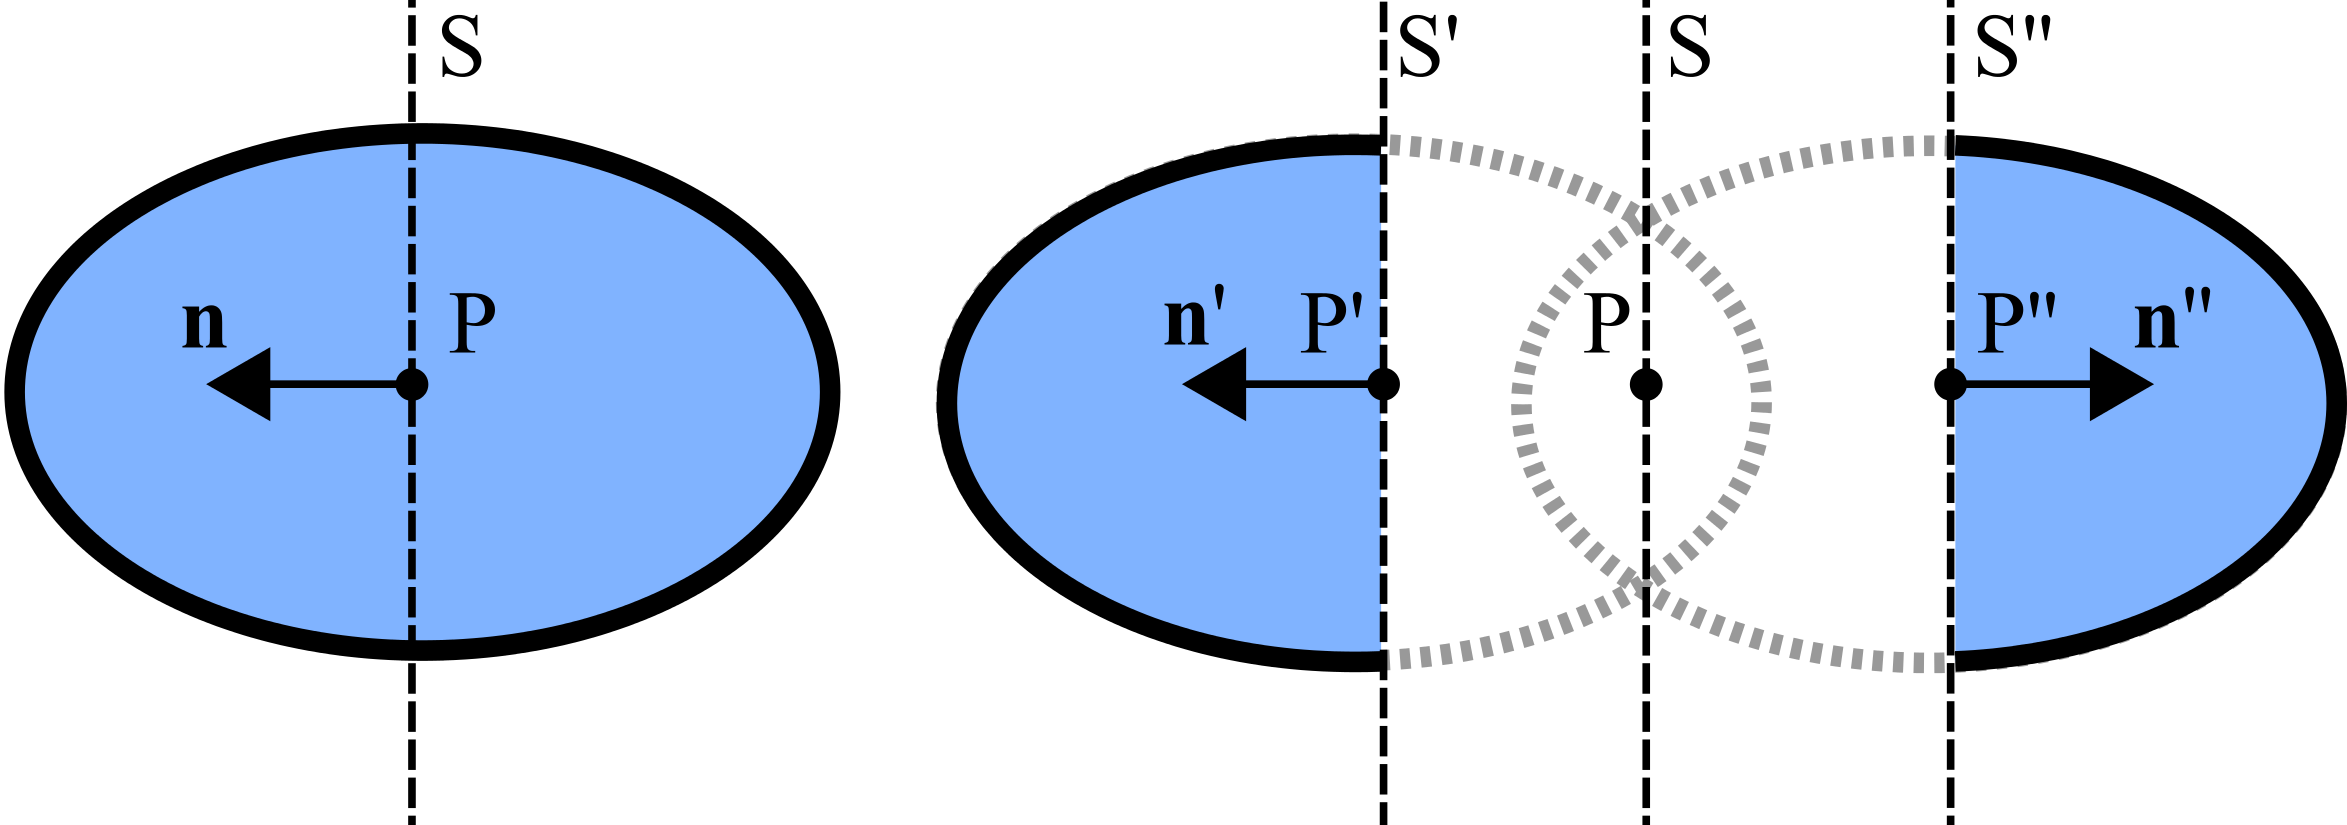
\includegraphics[width=0.9\textwidth]{chapters/figures/splitting_explained}
	\caption{The object is rendered twice with the parts behind the translated splitting planes $S'$ and $S''$ being ommited}
	\label{fig:splitting_explained}
\end{figure}
The first step towards an exploded view is not to split the whole object, but only the portions of it that are not the object of Interest. To do this, the already implemented group selection feature is used to define an object of interest that is not split and translated like the rest of the mesh. Before each rendering, the renderer now loops through the sections of the object and checks if they are part of the object  of interest. If the are not they are split and displaced as in the original plugin. For the interesting parts a third rendering of the mesh has been added to the display function. This render pass renders only the object of interest in its original location in the non-displaced mesh.\\
To draw the Object of interest the shader doesn't need to bother with split planes, backfaces and a displacement vector. Thus the shader is reverted to a basic triangle mesh shader when created with the options corresponding to the object of interest.\\
After that is done an exploded view of the object is now rendered with manual definition of the offset and split plane as seen in fig \ref{fig:cerebellum}. \\
One problem remains though: A colour picking algorithm was already implemented, which on a mouse click to the canvas. draws an overlay that has the group number encoded as an rgb color value. The color value at the click location is then instantly evaluated returning the the integer id of the selected part of the mesh. This works as designed but it doesn't conider that the mesh is now partially split and its parts may have been displaced. The result is that to select something, one has to click the location where it would be if it had not been displaced.\\
To set this right, the the overlay function was modified so that it would also be rendered three times like the normal rendering.
\begin{figure}[tb]
	\centering
	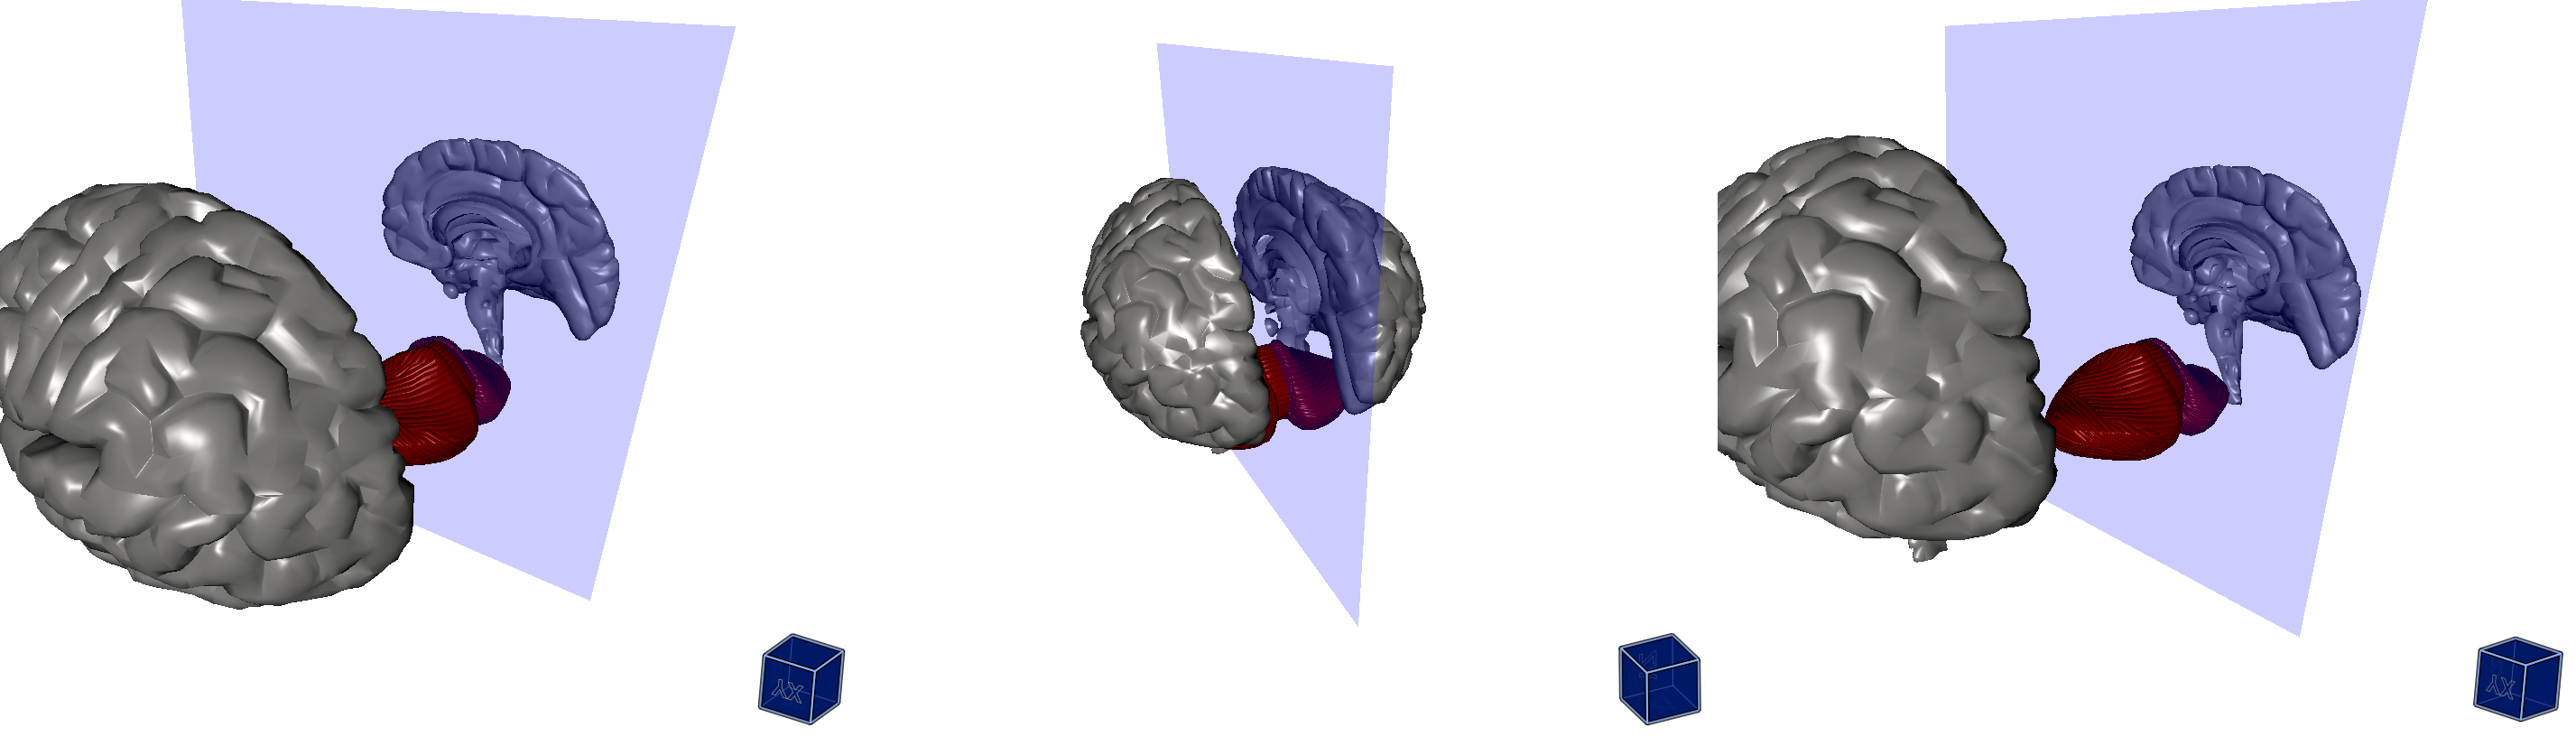
\includegraphics[width=0.9\textwidth]{chapters/figures/cerebellum}
	\caption{Exploded view of a brain with the offset of the displaced halves are set manually}
	\label{fig:cerebellum}
\end{figure}

\subsection{Milestone 2: find a safe distance, find a split plane} 
The next step is now to automatically displace place the two halves of the objectalong the explosion direction so that the object of interest is fully visible from every angle. To achieve this an animated displacement of the object has two big advantages over statically placing the objects at the safe distance:\\
\begin{itemize}
\item \textbf{Aesthetics} A smooth transition of an objects movement from one point to another is conceived as more ´´natural'' and therefore better-looking than an aprupt change of position. This conception can be reinforced by using animation techniques like slow in and slow out.\cite{misc:siggraph}
\item \textbf{Simplicity} Rather than finding the ideal distance by deterministically calculating it before displacing the object a much simpler approach is to guess such a distance by checkingif the object of interest is fully visible and then displacing the exploding parts otwards as long as this is not the case.
\end{itemize}
With these considerations in mind an implicit approach to finding the ideal offset of the two halves was used:\\
To see if the object is occluded it is drawn before the other objects that might occlude it and the number of pixels drawn to the screen is counted. Then, after the rest has been drawn the object of interest is drawn and its pixels are counted again. Because of the depth buffer, only the parts of the object that are not blocked from view are drawn, which means that if the both amounts of pixels from both renderings are the same the object is unoccluded.\\
To boost performance, the first rendering of the object of interest is done using the low cost overlay shader used in the color picking algorithm. Counting the rendered pixels of object of interest is done by using OpenGL queries. \\
Now it is possible to automatically generate an exploding view by making the offset of the exploding part grow until the object is fully visible. The offset grows at a constant speed which can be chosen in the user interface. If the object is unoccluded after a user interaction the offset shrinks until the first frame with a partial occlusion after which it grows again and stops when fully visible.\\ 
To achieve a more natural movement the relative amount of occlusion
\begin{equation}
	\label{eq:OcclusionRatio}
	r =\frac{p_{unoccluded} - p_{occluded}}{ p_{unoccluded}}
\end{equation}
for
\begin{equation}
	p_{occluded} \neq 0
\end{equation}
can be used to generate an ease-out-effect:
The speed is multiplied with $r$  specified by user input resulting in the speed, making the animation faster when little of the object of interest is visible and slower if much of it can be seen, coming to a halt as soon as the whole object is fully revealed which is the moment the ideal offset is set to the current offset.\\
This movement is akin to the movement of the object being pulled by a spring toward the point of full revelation of the object of interest, though not a linear spring, because the change of speed is determined by the amount of Pixels that are revealed in each iteration making the spring constant proportional to $r$.
To avoid that the Object still moves at very low speeds, resulting in huge amounts of unnecesary costly redraws, a minimum speed $\epsilon$ is introduced so that the object comes to a halt earlier.\\
\subsection{Milestone 3: Optimize Distance, force-field animation of split, optimize fringe distance cases} 
The objective of this last Milestone is to give a smooth appearance to the graphic while the view is changed by User interaction. The first step is to make the transition between two offsets smooth with the transition speed $s$ proportional to $\Delta_{offset}$
\begin{equation}
	s=s_u \cdot \Delta_{offset}
\end{equation}
thus creating a movement with linear deceleration that comes to a halt when the ideal offset is reached. this behaviour can be observed if the option ``Dynamic Offset `` is deactivated.\\
With dynamic ratio turned on and the object of interest is (partially) occluded the ideal offset is set to the maximum  offset and speed $s$ is multiplied by the ratio $r$ described in milestone 2 so that when the split parts move away from the object of interest the movement halts when the whole object is fully revealed setting the current offset as the ideal offset.\\
In case the object is revealed and the explosion needs to be collapsed the ideal offset is set to 0.0 until the object of interest is no longer fully visible, in which case the movement ideal offset is set to maximum and now grows outwards as described before.\\
This creates a visualization that smoothly adapts to new viewing points and changes in the splitting plane, but has one major disadvantage:\\
If a plane normal on either side of the plane points approximately in the same direction as the viewing vector,  the offset needed to reveal the whole object of interest become very huge in comparison to the object itself. This may prove fatal to the expressiveness of the visualization, given that the goal is to represent an object in context of the parts that are exploded, but the distance between the components is either so large that parts of the components partially move outside of the screen or even completely outside or behind the viewing plane or it is necessary to zoom out or move the camera back so that the whole object is visible causing substantial loss of detail, due to the large offset. If the $\vec{planeNormal} \cdot \vec{viewingVector} = \pm1$ or the object has a certain shape (e.g large at the end in direction of the offset, see  \ref{fig:infinity}
) the offset would even grow to infinity.\\
\begin{figure}[tb]
	\centering
	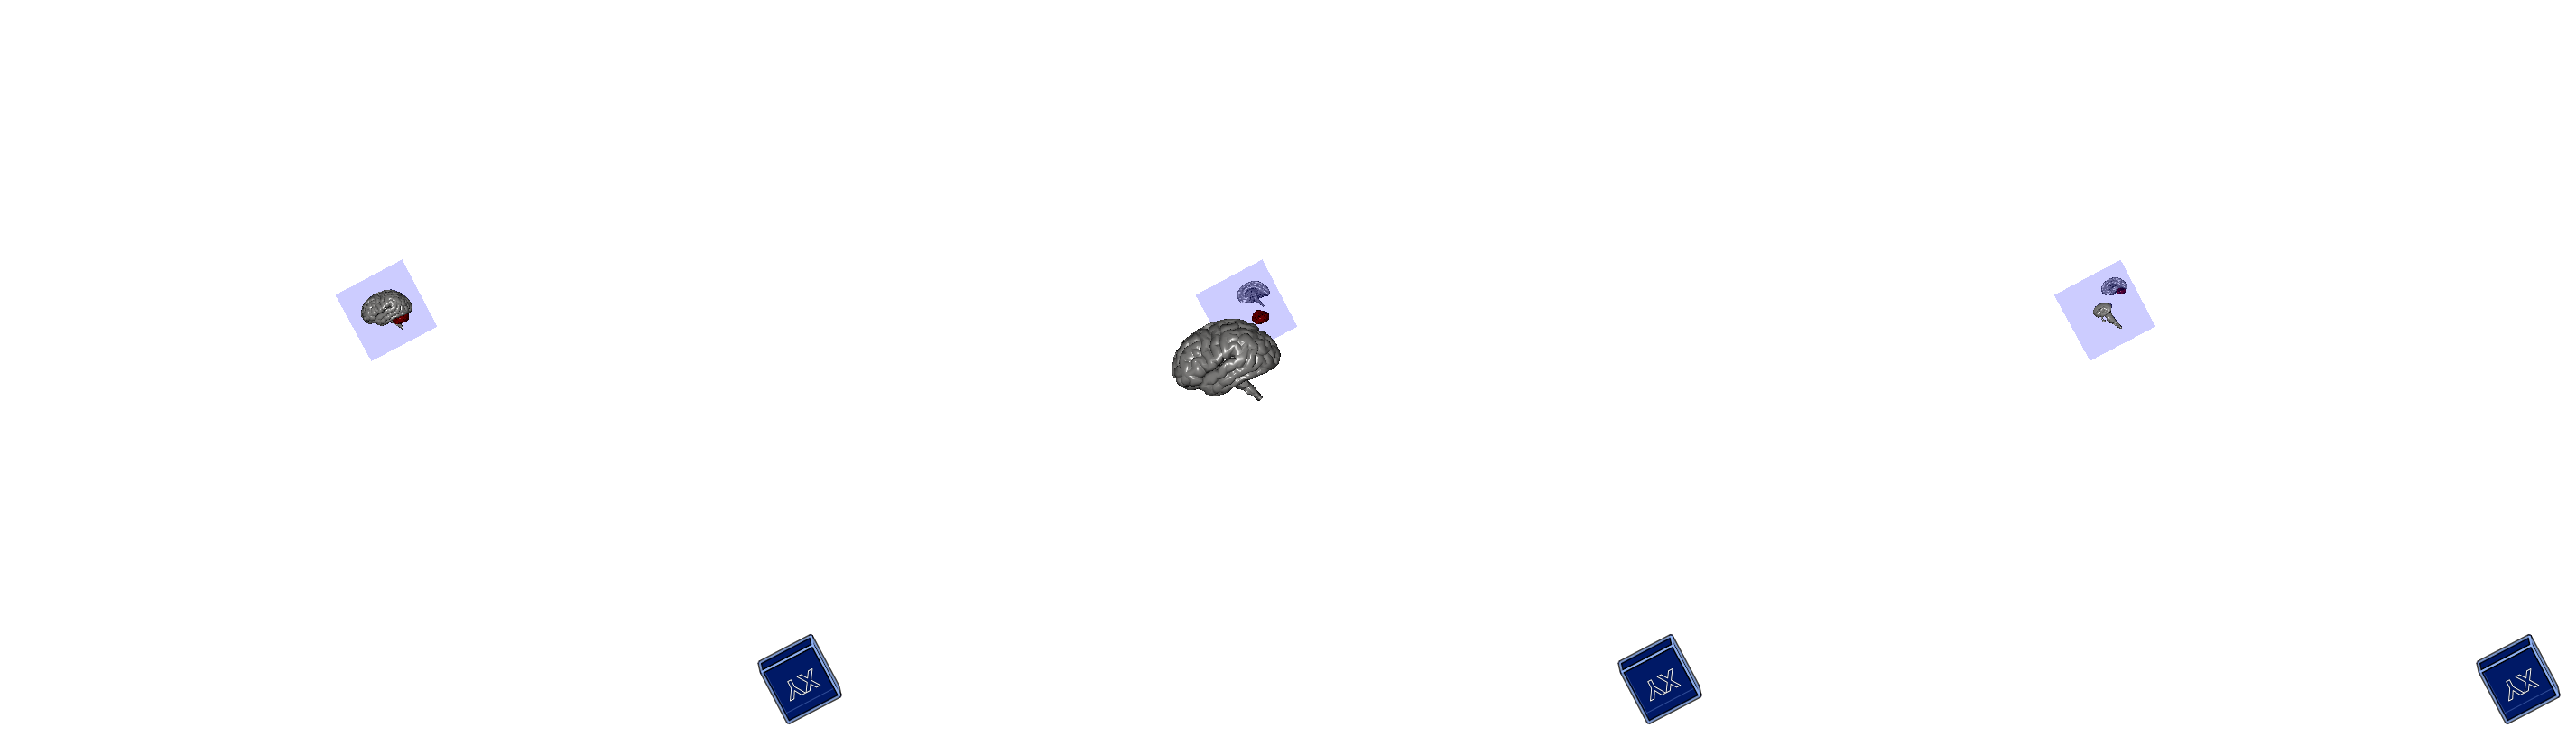
\includegraphics[width=0.9\textwidth]{chapters/figures/infinity}
	\caption{Different objects of interest from roghly the same viewpoint cause the offset to grow, placing the object out of view}
	\label{fig:infinity}
\end{figure}
To circumvent this problem I defined a maximum offset $o_{max}$ of the objects diameter which is the length of the distance between the minimum and maximum corners of the bounding box of the mesh. Since the mesh itself has no bounding box, the bounding box has to be accumulated by combining the bounding boxes of the groups of the mesh. This way the distance between the exploded parts can never exceed twice the diameter of the object.\\
To avoid parts of the object of interest now being occluded I used a simple ghosting technique: 
The front part, meaning the exploded part that is between the viewer and the split plane, is being rendered translucently if the distance becomes too large.
If the current offset $o_c$ exceeds $o_{max} \cdot 0.7$ the opacity $\alpha$ of the front part is linearly interpolated between $1.0$ at $o_c = o_{max} \cdot 0.7$ and $0.5$ at  $o_c = o_{max}$ using the formula
\begin{equation}
	\alpha = \frac{o_{max}-o_c}{o_{max} \cdot 0.3} \cdot 0.5 + 0.5
\end{equation}
This opacity factor $\alpha$ is then multiplied by $r$ \ref{eq:OcclusionRatio}  so that the object stays solid while its not occluding anything and is most translucent if the whole object of interest is occluded completely.\\
\begin{verbatim}
//get the occlusion ratio
float ratio_selected = occlusions[0]- occlusions[1];
	if (ratio_selected>0){
	ratio_selected/=occlusions[0];
	
	// set the offset
	if (ghosting){
		ideal_offset[0]=boundsDiameter;
		ideal_offset[1]=-boundsDiameter;
	}else{
		ideal_offset[0]=20.0f;
		ideal_offset[1]=-20.0f;
	}
	
	//multiply the ratio to the speed
	speed=GetPlugin().GetProperty("Speed");
	speed*=ratio_selected;
}else{
	//stop
	}
\end{verbatim}
To determine which part is the front part, I calculated the dot product of the viewing vector and the plane normal, using its sign to determine whether the part shifted in direction of the plane normal is the front part or not. This also determines in which order the parts are rendered, with the front part being the last, so that it can be translucently blended over the solid parts.\\
A problem that now appears is that backface culling is deactivated to so that the cutaway can be rendered correctly, resulting in the translucent objects' backfaces also visible, which causes the graphic to appear slightly confusing and aesthetically unpleasant. This can be avoided by allowing backface culling for a translucent object, if its offset vector doesn't point away from the camera. Because this may be the case if the camera is placed between the original and the translated switch plane, the dot product has to be calculated once more, now for the translated split plane.\\
\begin{figure}[tb]
	\centering
	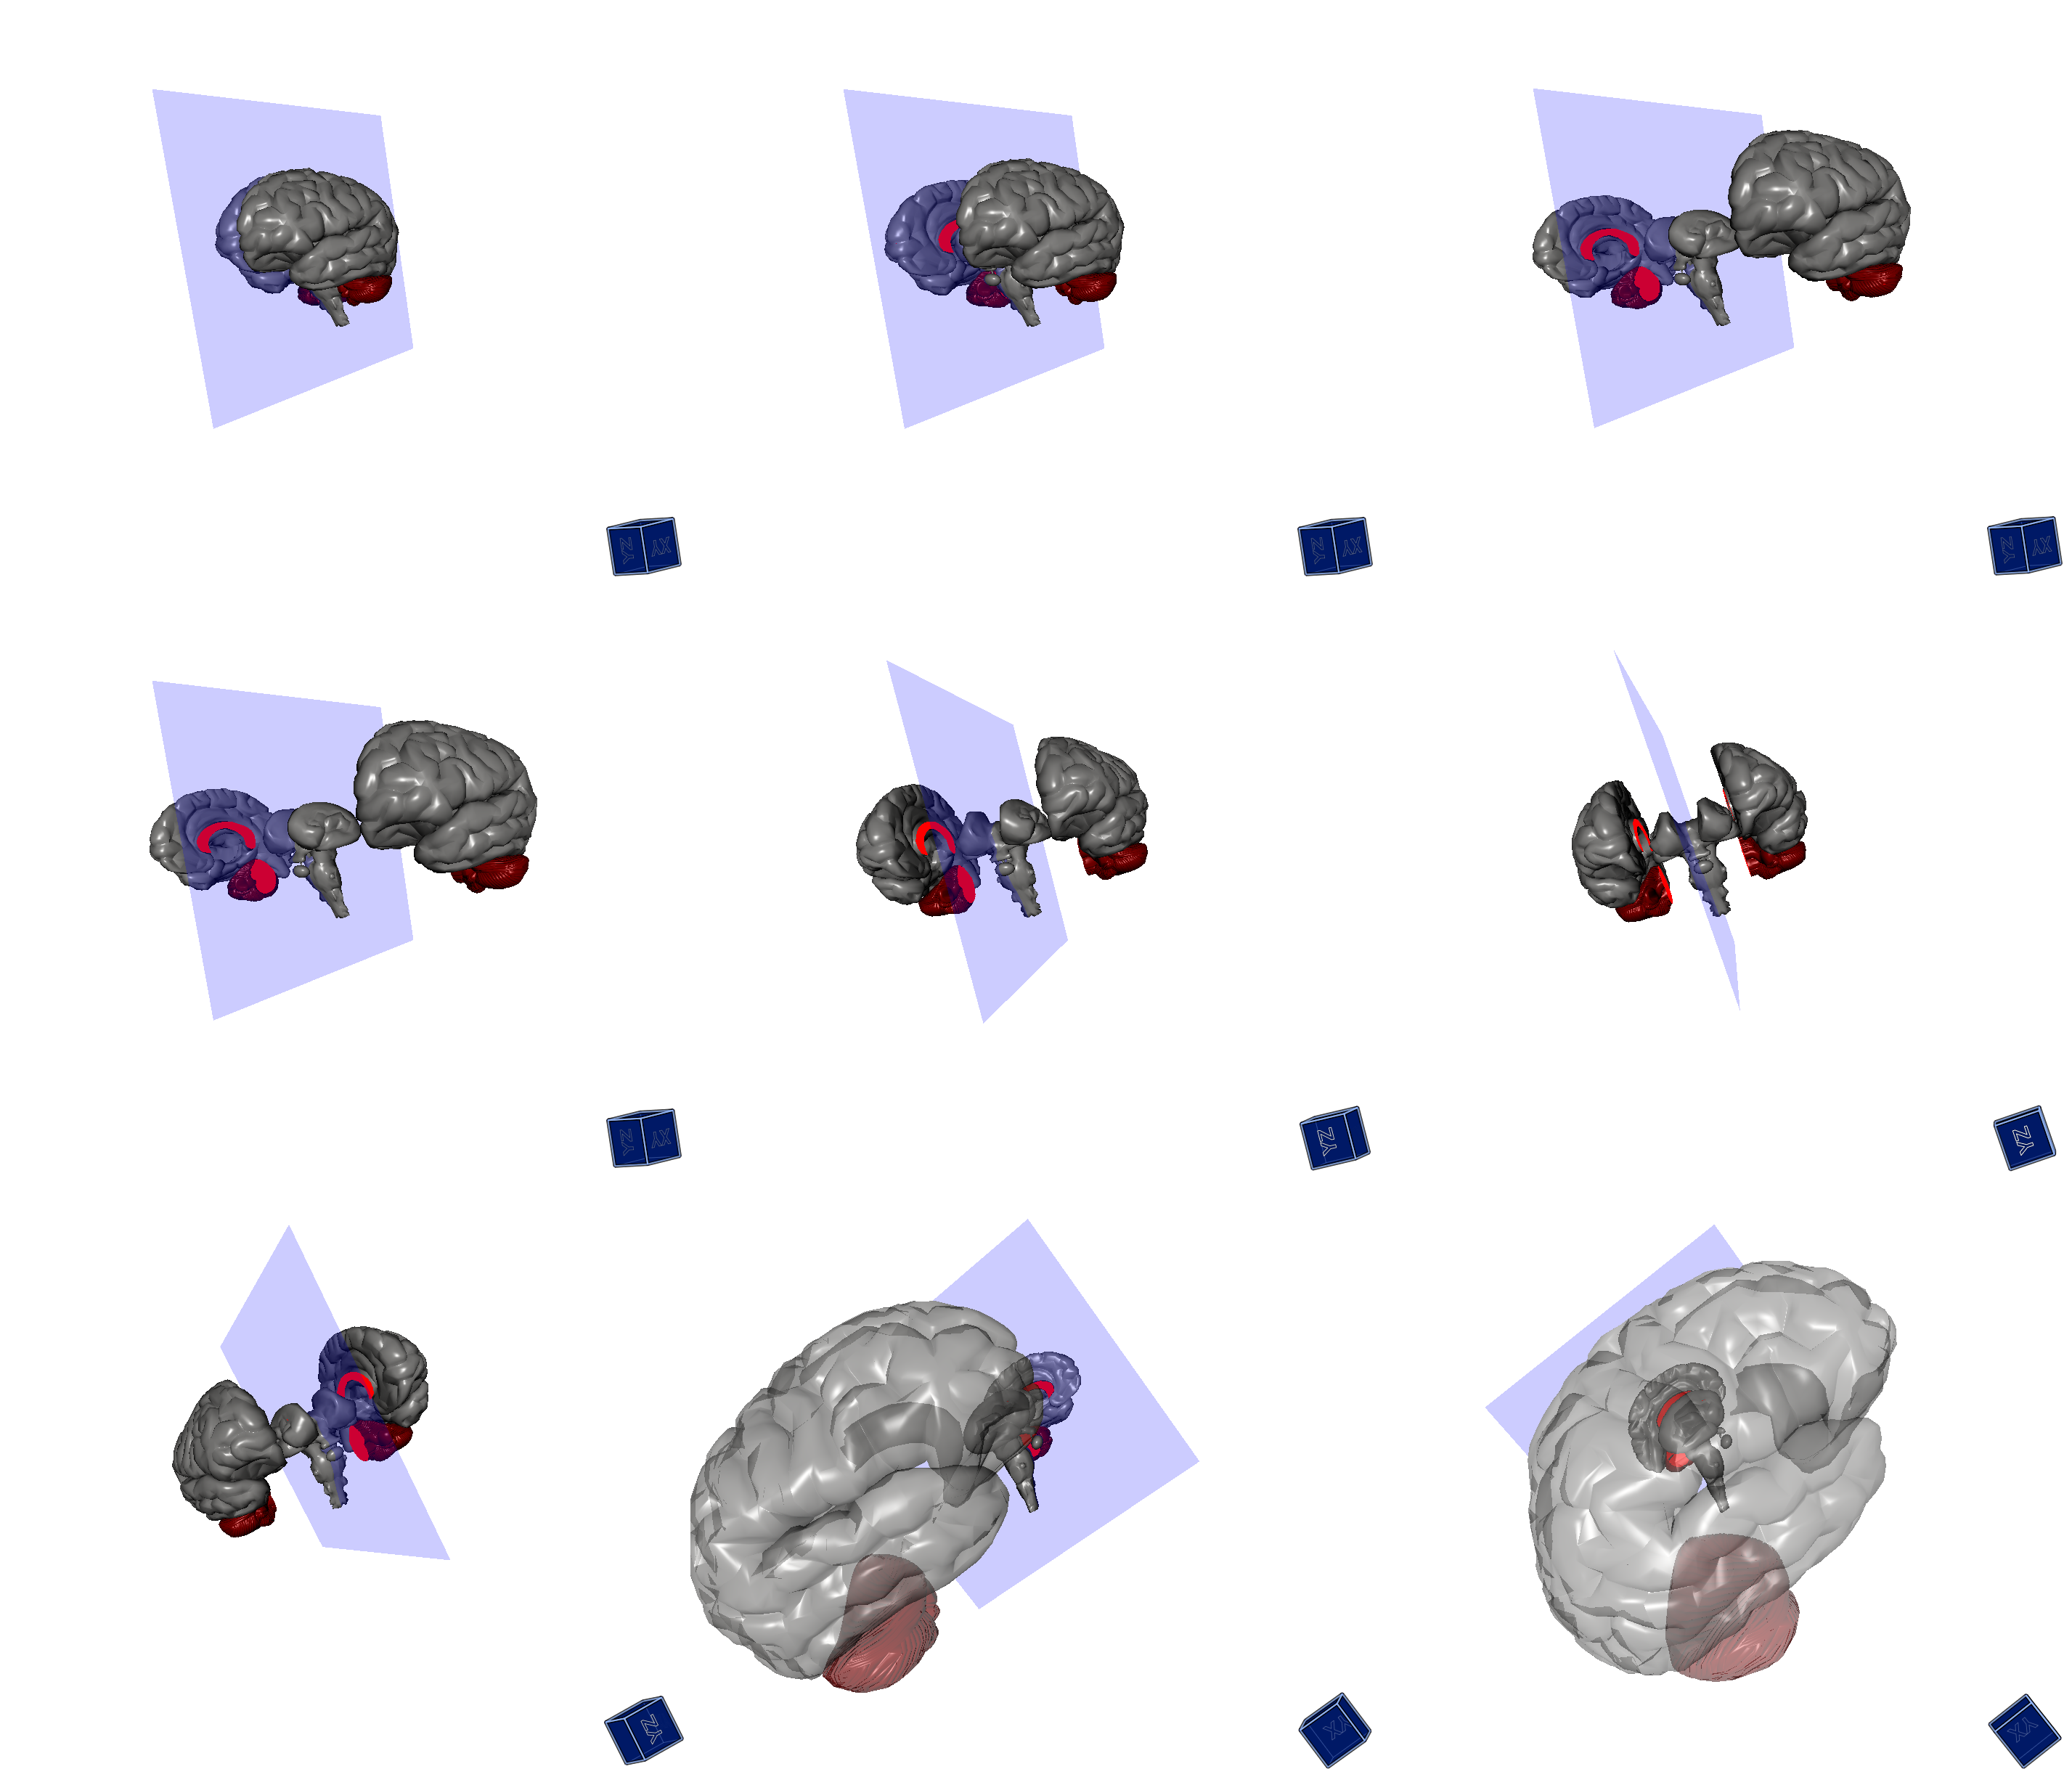
\includegraphics[width=0.9\textwidth]{chapters/figures/brainstem}
	\caption{Depiction of the animations and ghosting in the final version of the plugin}
	\label{fig:brainstem}
\end{figure}
\chapter{Conclusion}
In general I think that the combination of ghosting and exploded views is an improvement upon the technique of exploded views.  In comparison to the behavior the pure explosive view exhibits when viewed from angles close to the explosion direction it gives more information about the object of interest and it looks better than a solid part blocking it or disappearing from view.\\
Ghosting on the other hand loses one of its key advantages, namely that all parts of the object appear in their original location.
\subsubsection{Future Work}
At the moment the explosive view is very basic, with the explosion only along one axis, and a hierarchy that consists of only  an object of interest and its context objects. The next steps to imrove uüpon the visualisation would be to introduce more levels into the part hierarchy and devise a way to explode along mutible axes and exploring ways to quasi-naturally animate these behaviours.